\chapter{Achieved Results}\label{chap:results}

This chapter sums up the results achieved so far. Section \ref{platform}
describes the design of the RoFI evaluation platform and reports current
progress. Section \ref{smt} describes our experiments on solving the
reconfiguration problem via reduction to SMT.

\section{RoFI Platform}\label{platform}

We developed \emph{RoFI} -- a new platform of distributed metamorphic robots
that is open-hardware and open-source, hence almost freely available to anyone
interested. We designed our metamorphic robotic platform on top of the actual
results of other teams, and in a way, that other researchers may easily create a
physical copy of the platform on their own. We provide enough documentation to
mitigate the challenge of software development for the platform, and we
encourage others to use our platform to demonstrate the results of their work.
We believe a general publicly available platform for metamorphic robots is
beneficial for the whole community. It will prevent others from reinventing the
wheel while producing their robots and research results.

The RoFI platform is hybrid type -- its modules are designed to fit inside a
regular cubical grid. It does not define a single module shape, but it allows
the users to define custom module shapes if desired. We put several constraints
on the module shape to make the modules \emph{grid-aware} -- see Figure
\ref{fig:gridAware}. Grid-awareness allows for easier reconfiguration in dense
configurations and also combines the advantages of both lattice type and chain
type self-reconfigurable robots. This versatility is one of the contributions of
the platform.

\begin{figure}[t]
    \centering
    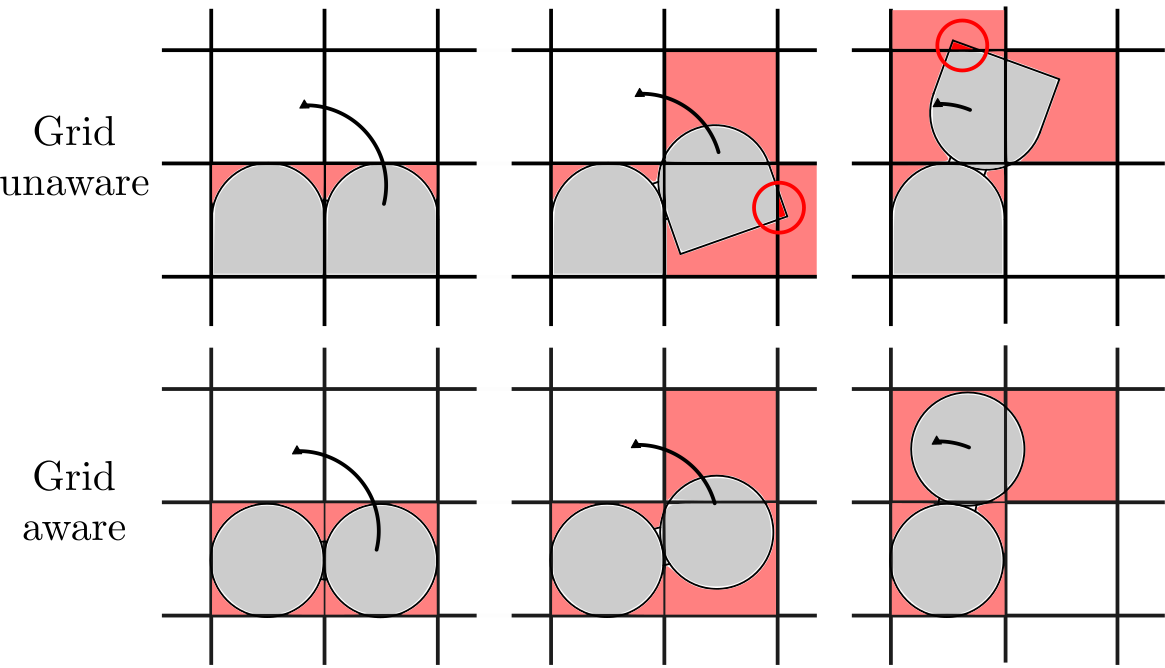
\includegraphics[width=0.7\linewidth]{figures/grid_aware.pdf}
    \caption{Illustration of grid-awareness (sequence in time). If
    a double cell module tries to move one of its bodies from right to top, the
    grid-unaware module occupies extra cells of the grid.}
    \label{fig:gridAware}
\end{figure}

However, the grid-awareness comes at the cost of the increased complexity of the
connector mechanism as it needs to be retractable. Therefore, we developed a
connector suitable for this task: RoFICoM. We give more details about it in
Section \ref{connector}.

We designed the inter-module communication such that it feeds various needs of
researchers. RoFICoMs offer point-to-point connection, which is suitable for,
e.g., digital hormone control. If broadcast, module-to-module communication, or
remote control is needed, we integrated RoFICoMs as another physical layer to
the popular lwIp library~\cite{lwip} implementing TCP/IP stack. Therefore, our
modules can easily interact with existing computer networks. To do so, we
designed a way for module IP address autoconfiguration and packet routing.

We demonstrate the proposed RoFI platform specification on the \emph{universal
module} (see Figure \ref{fig:umPhoto}). The universal module is a 2-cell module
inspired by M-TRAN. Unlike M-TRAN it has an additional joint in the middle to
allow for more versatile reconfiguration and control (e.g., the loop
configuration can steer via this joint). The module can sense torque on all of
its axes, features an inertial measurement unit, and the connectors are capable
of time-of-light distance measuring, which serves to scan of the
surrounding environment.

\begin{figure}[t]
    \centering
    \includegraphics[width=0.8\linewidth]{figures/um_persp.jpg}
    \caption{Photo of a single universal module.}
    \label{fig:umPhoto}
\end{figure}

Our goal is to provide means for the user to develop control software for RoFI
modules either in C++ or Python without the burden of a variety of low-level
technical issues. Therefore, we provide a set of high-level drivers and
libraries to control them. We would also like to allow users to easily validate
their software without the hassle of dealing with physical robots. We provide
simulation software that can directly execute the module firmware in a virtual
environment.

The whole software architecture is depicted by Figure~\ref{fig:architecture}.
The bottom layer is the \emph{hardware abstraction layer} (HAL). HAL is a set of
C++ functions, that control the basic module capabilities directly related to
the hardware, e.g., controlling joints, reading sensors, or sending messages via
connectors. All the other layers rely on HAL.

\emph{RoFI Operating System} (RoFIOS) operates on top of HAL. RoFIOS covers
essential functionality that practically all user programs rely on and is
supposed to be opaque to the user. It includes, e.g., implementation of
networking (packet routing, address mapping), module identification and
discovery, logging, firmware updates, or remote calls to the RoFIOS interface on
another module.

Directly on top of the RoFIOS runs the user firmware, which can be written
either in C++ (the preferred way) or Python. The Python programs are executed
using the MicroPython interpreter\footnote{\url{https://micropython.org/}}. User
programs do not have to be self-contained. We provide a collection of libraries
the user can use. These libraries are continuously growing and cover, e.g.,
functionality related to distributed control, environment sensing,
reconfiguration, and more.

\begin{figure}[t]
   \centering
   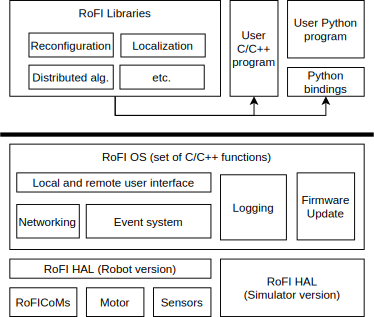
\includegraphics[width=0.7\linewidth]{figures/architecture.pdf}
   \caption{Overview of the software architecture of the RoFI platform.
   Components above other components strictly depend on them. The thick
   horizontal line defines the border between essential runtime provided by the
   modules and user programs.}
   \label{fig:architecture}
\end{figure}

The introduction of HAL allows to simulate programs for RoFI easily -- the users
just have to compile their program with the simulator version of HAL. We have
developed a plugin for Gazebo~\cite{Gazebo}, which allows simulating multiple
robots, including their distributed nature -- a crash of the user program does
not cause a crash of the simulation. See Figure \ref{fig:gazebo}.

\begin{figure}[!t]
    \centering
    \begin{subfigure}[b]{0.45\textwidth}
        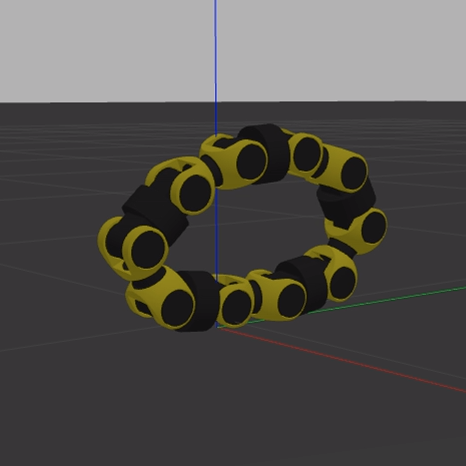
\includegraphics[width=\textwidth]{figures/sim-roller.png}
        \caption{Loop configuration}
    \end{subfigure}
    ~
    \begin{subfigure}[b]{0.45\textwidth}
        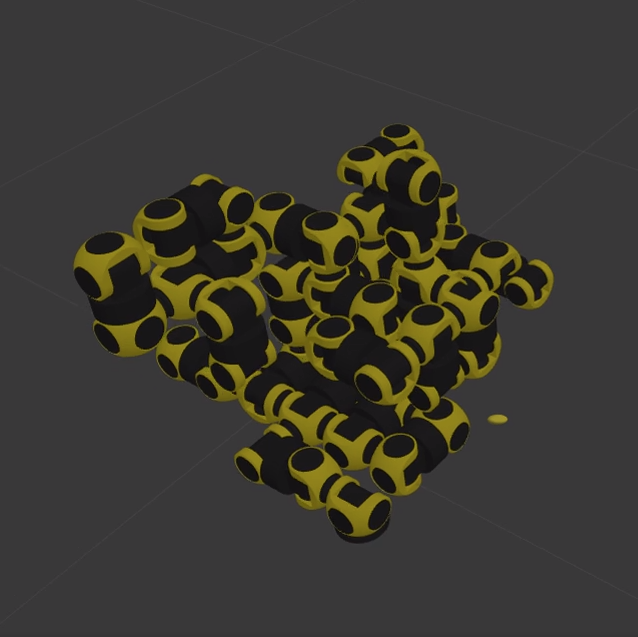
\includegraphics[width=\textwidth]{figures/sim-large.png}
        \caption{50 modules under simulation}
    \end{subfigure}

    \caption{Examples of configuration loaded into the Gazebo simulator.}\label{fig:gazebo}
\end{figure}

The publication of the RoFI platform as a whole is currently in progress. I am
the author of the RoFI platform design -- the module shape descriptors, I also
developed the hardware and software of the universal module of the platform. The
ecosystem around RoFI was developed by students working on the project under my
guidance and assistance.

\section{RoFICoM}\label{connector}

RoFICoM is a genderless, 4-ways symmetrical connector for grid-aware robots that
allows for mechanical connection between two modules. See Figure
\ref{fig:roficom} for the photo of the connector. The connector also establishes
data communication and power-sharing between the modules. It is an encapsulated
device that can be easily reused in various module types. To our knowledge, it
is the only connector that comes in the form of an encapsulated device, which is
easy to integrate and is open-hardware and open-source. The connector is not
only comparable with state-of-the-art in the aspects of speed and strength, but
it also outperforms it in the offered features (e.g., passive counterparts) and
miniaturization.

\begin{figure}[t]
    \centering
    \includegraphics[width=0.8\linewidth]{figures/connector_photo.jpg}
    \caption{Photo of RoFICoM.}
    \label{fig:roficom}
\end{figure}

The RoFICoM design was already published \cite{DBLP:conf/iros/MrazekB19} (full
paper version is attached at the end of this thesis). The whole RoFICoM design
(including hardware, electronics, and firmware) is my design.

\section{Reconfiguration via Reduction to SMT}\label{smt}

One of the possible approaches to finding a reconfiguration plan is based on the
exploration of the system's state-space. This approach is rather infeasible
without further heuristics as the state-space of all possible transformations is
vast. The state-space exploration is a widely used technique also in the field
of formal verification. In this field, recently, many tools stopped directly
exploring the state-space of a system, and instead, they are reducing the
problem to the problem of \emph{satisfiability modulo theory}
(SMT)~\cite{DBLP:series/faia/2009-185}. In a nutshell, the verification tool
constructs a logic formula such that it is satisfiable if and only if the
erroneous state of the system under inspection is reachable. After that, the
formula is passed to an SMT solver, which decides its satisfiability. The
SMT-reduction based approach has proven to be quite effective in the
verification community as it leverages the sophisticated heuristics implemented
in the solvers.

In this work, we explore the possibility of applying a similar approach -- we
want to leverage SMT and SMT solvers to tackle the problem of reconfiguration.
Our basic goals are twofold: first, to find out whether the suggested way is a
viable one in terms of practical usability, and second, to see how much of a
performance boost we can expect in the future from the continuous development of
SMT solvers. Compared to work by \textcite{DBLP:journals/pcs/GorbenkoP12}, our
approach yields collision-free reconfiguration plans.

The \emph{reconfiguration plan} for two configurations $c_{initial}$ and
$c_{target}$ is a~sequence $(c_{initial}, c_2, \cdots, c_{n - 1}, c_{target})$
of configurations such that all configurations are strongly connected (as we
model modules without locomotion) and also for every two consecutive
configurations $c_i$ and $c_{i+1}$ it holds that either they are the same or
$c_{i+1}$ can be obtained from ${c_i}$  by applying exactly one of the following
actions: releasing some connections, establishment of new connections, or
joints' movement.

Let us assume that we can construct a first-order formula
$\pi_{n}(c_{initial}, c_{target})$ in the theory of non-linear real arithmetic
such that the $\pi_n$ is satisfiable if and only if there exists a valid
reconfiguration plan of length $n$ from $c_{initial}$ to $c_{target}$. Then we
can pass $\pi_n$ to an appropriate solver and find out whether it is satisfiable
or not. If so, we can easily extract the reconfiguration plan from the model of
the formula.

To find the shortest path, we may iteratively construct $\pi_2$,
$\pi_3$, $\pi_4$, $\cdots$ to find out the first satisfiable formula. The
possible improvement of this naive approach would be to guess an upper bound on the
length of the shortest reconfiguration plan and use binary search to find the
lowest $n$ for which $\pi_n$ is satisfiable.

The challenge of this approach lies in the construction of $\pi_n$. In our work,
we tested several approaches for expressing the formula. We tackle it by
introducing a concept of the \emph{external} and \emph{internal} representation
of a~configuration. The internal representation provides a trivial way to
encode a transition from one configuration to another; the external provides a
trivial ways encoding configuration validity. Therefore, we only need to express
a~relation between these two representations in the logic. The naive
expression does not work as the formula is large and state-of-the-art solvers
struggle with trigonometry. We solve this problem by using quaternions to
express modules' orientation. We also propose a suitable discretization to
circumvent the need to use an universal quantifier as the solvers do not handle
universal quantification.

We evaluated our work on several version of the following solvers Z3
\cite{DBLP:conf/tacas/MouraB08}, SMTRAT \cite{DBLP:conf/sat/CorziliusKJSA15},
dReal \cite{DBLP:conf/cade/GaoKC13}, Yices2 \cite{DBLP:conf/cav/Dutertre14},
CVC4 \cite{DBLP:conf/cav/BarrettCDHJKRT11}. Based on our experimental
evaluation, our approach is comparable to the existing state-of-the-art in this
area and, therefore, is currently inapplicable in practice. However, during the
evaluation of the historical version of the solvers, we noticed performance
improvements between the versions. Thus this approach might be viable in the
future.

Publication of this work is currently in progress. I am a co-author
of the core idea, I am the author of the quaternion-based optimization. I also
created a reference implementation and I performed the experiments.

\section{Publications}

\begin{itemize}

    \item \fullcite{DBLP:conf/iros/MrazekB19}

    I am the main author of the design and paper text.
\end{itemize}